\section{Spectacle (3 points)}

Pour le spectacle de fin d'année, la maîtresse a placé 7 élèves de ma classe de CE2 comme sur le schéma ci-dessous.

\begin{center}
	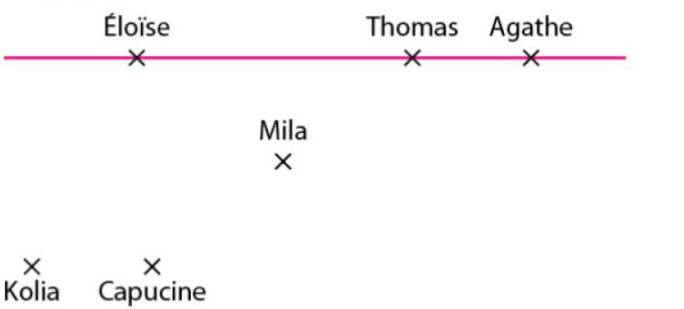
\includegraphics[scale=0.5]{img/spectacle}
\end{center}

Elle veut que la position des élèves soit symétrique par rapport à celle de Mila.

\begin{questions}
	\question[1\half] En utilisant uniquement une règle non graduée, déterminer la position d'Eneko, le dernier élève à ne pas avoir encore été placé. Laisser apparents les traits de construction.
	
	\begin{solution}
		\begin{center}
			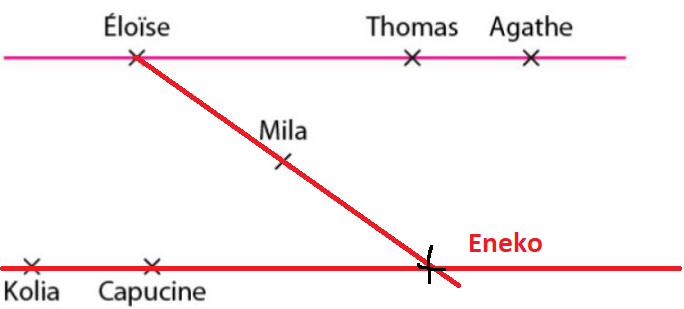
\includegraphics[scale=0.5]{img/spectacle_corr}
		\end{center}
	\end{solution}
	
	\question[1\half] Quelle propriété permet de répondre à la question ?
	\begin{solution}
		On sait que \'Eloïse, Thomas et Agathe sont alignés,
		or le symétrique d'une droite par rapport à un point est une autre droite. 
		Donc Kolia, Capucine et Thomas seront aussi alignés.
	\end{solution}
\end{questions}